\documentclass[10pt, a4paper,spanish]{article}

\usepackage[utf8]{inputenc}
\usepackage[spanish]{babel}

\usepackage[T1]{fontenc}

\usepackage[hmarginratio=1:1,top=32mm,columnsep=20pt]{geometry}
\usepackage[hang, small,labelfont=bf,up,textfont=it,up]{caption}

\usepackage{float}

\usepackage{amsmath}

\usepackage{graphicx}
\graphicspath{ {images/} }



\usepackage{abstract}
\renewcommand{\abstractnamefont}{\normalfont\bfseries}
\renewcommand{\abstracttextfont}{\normalfont\small\itshape}


\usepackage{titlesec}
\renewcommand\thesection{\Roman{section}}
\renewcommand\thesubsection{\Roman{subsection}}
\titleformat{\section}[block]{\large\scshape\centering}{\thesection.}{1em}{}
\titleformat{\subsection}[block]{\large}{\thesubsection.}{1em}{}

\usepackage{fancyhdr}
\pagestyle{fancy}
\fancyhead{}
\fancyfoot{}
\fancyhead[C]{ \today \ $\bullet$ Minería de Datos $\bullet$ Redes de Elman y Jordan}
\fancyfoot[RO]{\thepage}

%-------------------------------------------------------------------------------
%	TITLE SECTION
%-------------------------------------------------------------------------------

\title{\vspace{-15mm}\fontsize{24pt}{10pt}\selectfont\textbf{Redes de Elman y Jordan}} % Article title

\author{García Prado, Sergio}
\date{\today}

%-------------------------------------------------------------------------------

\begin{document}

	\maketitle % Insert title

	\thispagestyle{fancy} % All pages have headers and footers


%-------------------------------------------------------------------------------
%	ABSTRACT
%-------------------------------------------------------------------------------

	\begin{abstract}
		\noindent Abstract del documento
	\end{abstract}

%-------------------------------------------------------------------------------
%	TEXT
%-------------------------------------------------------------------------------


  \section{Introducción}

      \paragraph{}

	\section{Redes de Elman y Jordan}

			\paragraph{}

			\subsection{Encaminamiento hacia adelante}

				\paragraph{}

			\subsection{Encaminamiento hacia atrás}

				\paragraph{}

			\subsection{Diferencias}

	\section{Implementación}

		\paragraph{}

	\section{Resultados}

		\begin{figure}[H]
			\begin{center}
				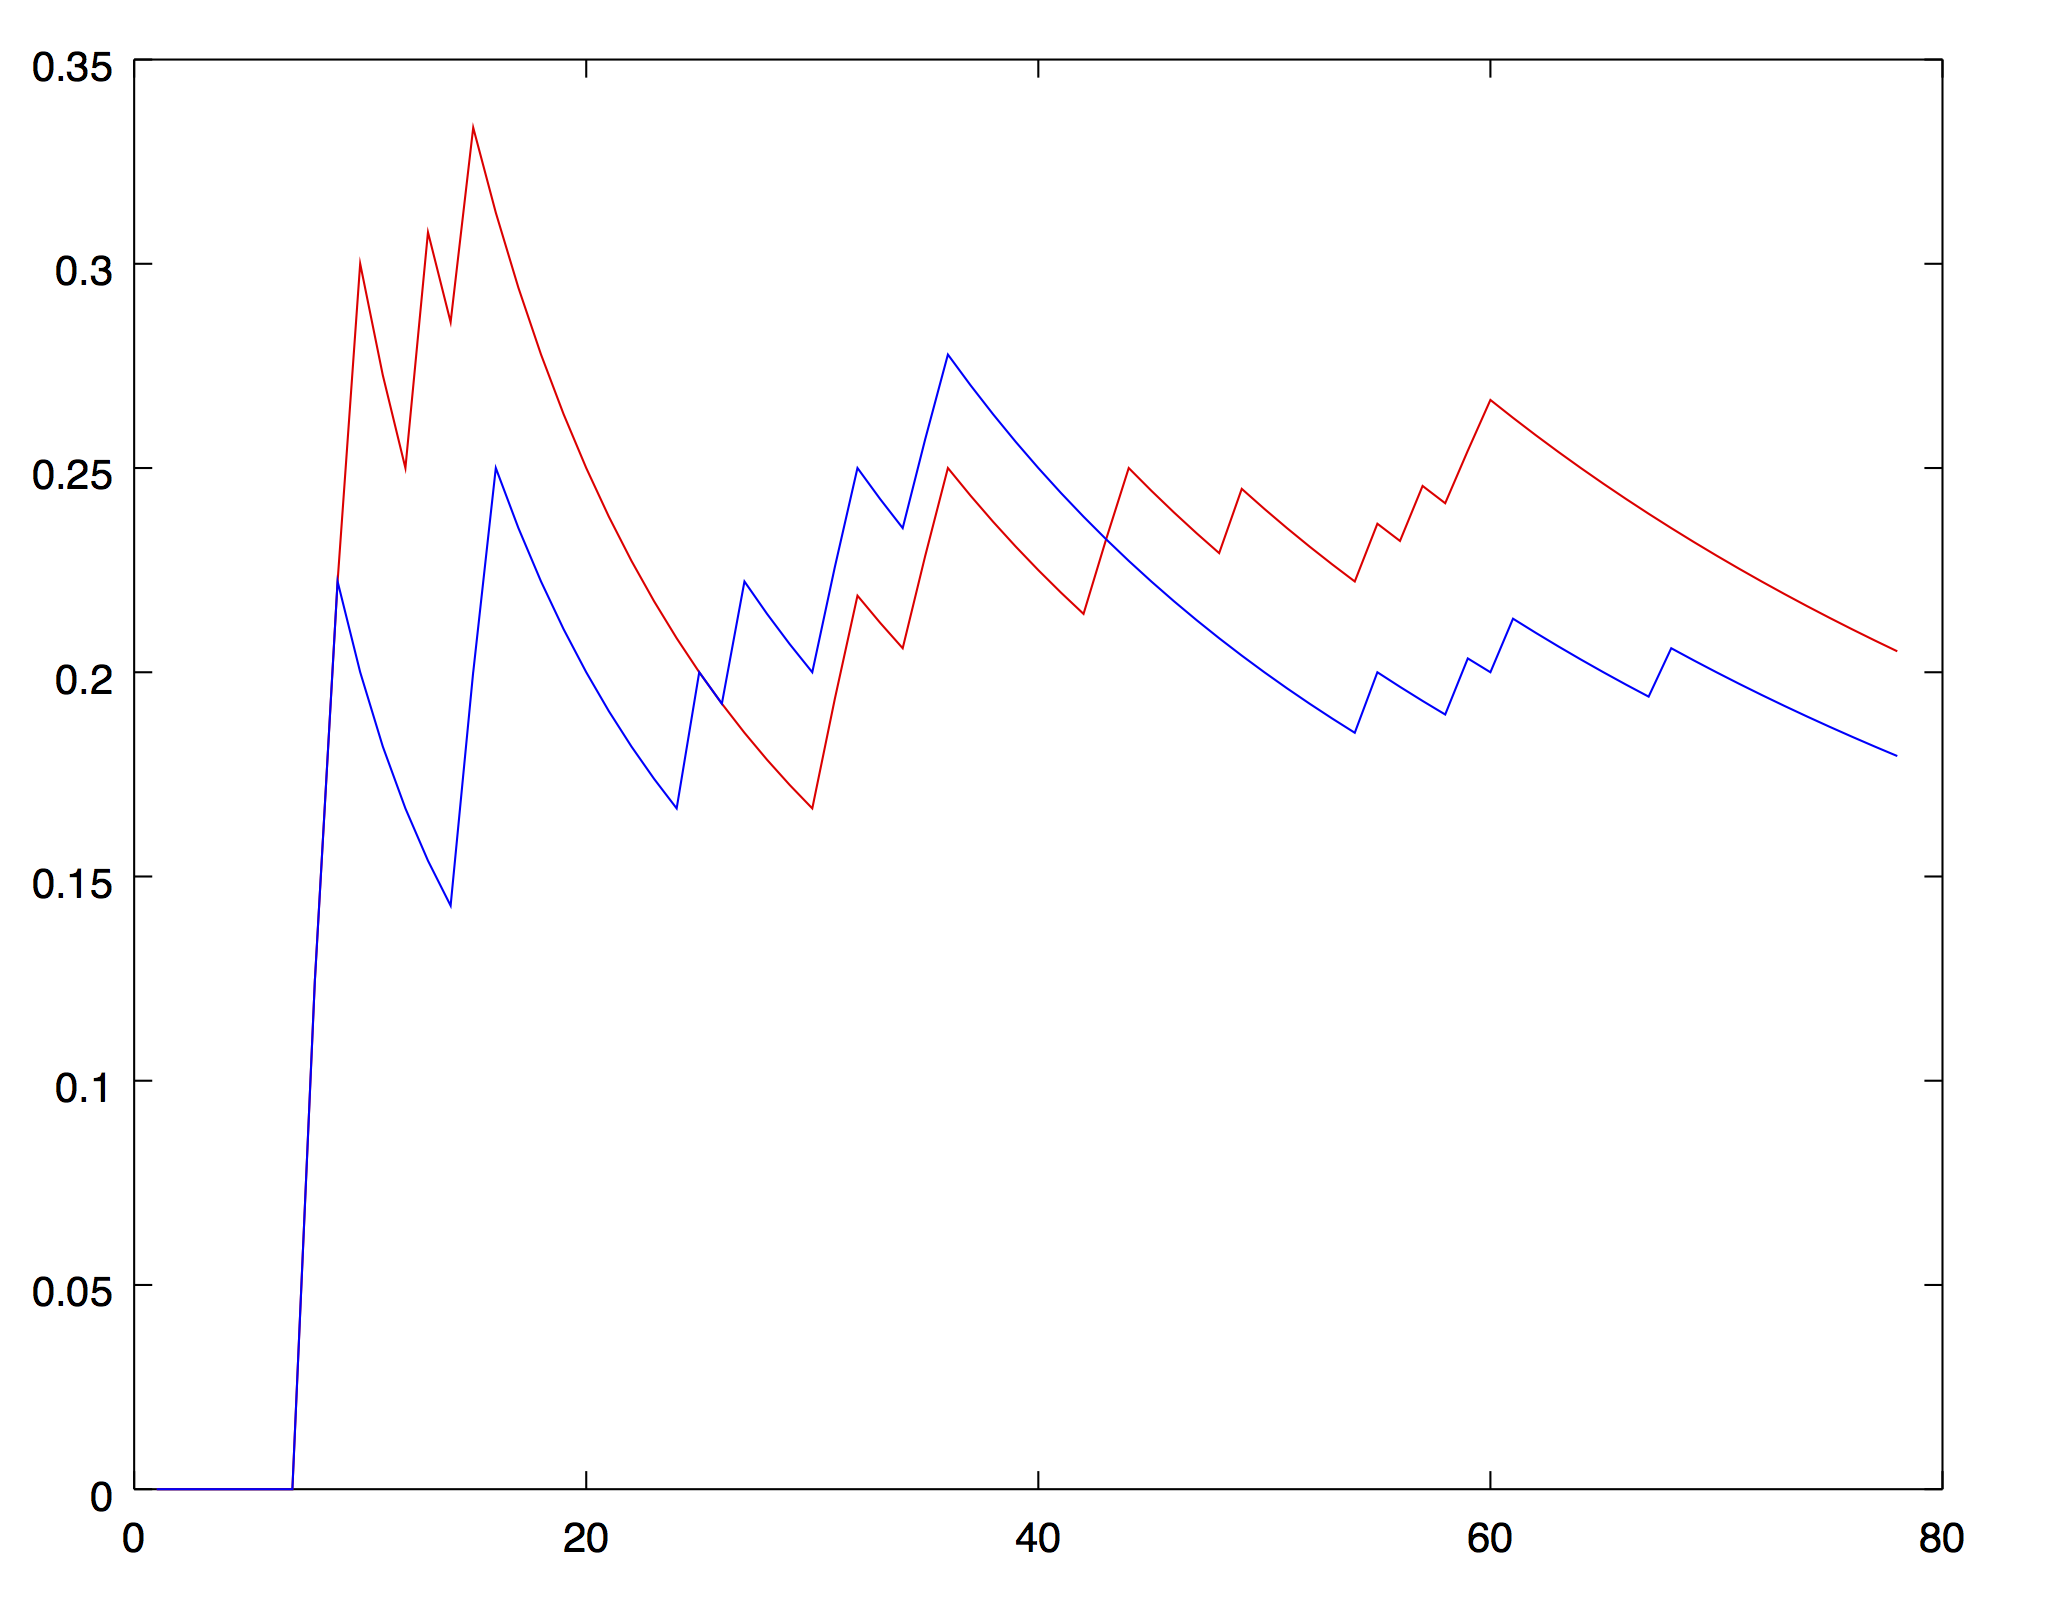
\includegraphics[width=0.9\textwidth]{chart}
			\end{center}
		\end{figure}

		\paragraph{}

\end{document}
